% *- coding: UTF-8 -*-
% !TEX builder = Texlive
% !TEX prggram = xelatex
\documentclass[UTF8,a4paper,12pt,titlepage]{ctexart}
% tittlepage制作一个封面
% draft是草稿,有个方框
%\documentclass[UTF8,a4paper,11pt]{book}

%\CTEXsetup[name={第,章}]{section}%每section统一名称

%每章节题目统一格式
\CTEXsetup[format={\zihao{-3}\raggedright\bfseries}]
{section}

\newcommand{\keyword}[1]{\textbf{#1}}

%\usepackage{microtype}

% 纸张格式
\usepackage[paper=a4paper,inner=1.5cm,outer=2cm,top=2cm,
bottom=2.5cm,bindingoffset=0.5cm]{geometry}

\usepackage[onehalfspacing]{setspace} % 1.5倍行距

% 自动链接内容
\usepackage[colorlinks=true,linkcolor=black]{hyperref}
% 设置文件属性内容
\hypersetup{pdfauthor={吴毓明},
            pdftitle={高锰酸钾自动制备投加装置},
            pdfsubject={使用说明},
            pdfkeywords={任何问题,联系61508712@qq.com}}

% 定义页眉页脚
% 定义页眉页脚
\usepackage{fancyhdr}
\fancyhf{}
\pagestyle{fancy}
% 公共
\rhead{\zihao{6}一体化全自动加药装置/化工泵\\
       Manage Pump as Diamond} % 页眉右

% 利亨昌
% \lhead{
\includegraphics{LHC-head.png}}% 页眉左
% \lhead{
\includegraphics[height=0.5cm]{LHC.jpg}} % 页眉左
% \chead{\zihao{4}广州市利亨昌贸易有限公司}
% \chead{\zihao{5}广州市利亨昌贸易有限公司}
% \lfoot{\zihao{6}广州市荔湾区东联路2号工业园\\
%                电话:020-8430 1397 传真:020-84301170 \\ 
%                电邮:gzlhcmy@163.com 网址:www.lhcmy.com}
% \cfoot{\thepage} % 页脚右
% \cfoot{\zihao{5}\thepage} % 页脚中
% \rfoot{\zihao{6}美国帕斯菲达PULSAFEEDER 产品库存商\\Paddle-flow流量监控及加药装置} % 页脚右
% \rfoot{\zihao{6}美国帕斯菲达PULSAFEEDER 产品库存商\\Paddle-flow流量监控及加药装置} % 页脚右
% \rfoot{\thepage} % 页脚右

% paddle-flow
%\rhead{\includegraphics{paddle-flow.png}}

% 厦门飞华
\lfoot{厦门飞华环保有限公司}
\rfoot{\thepage} % 页脚右



\renewcommand{\headrulewidth}{0.4pt} % 页眉分隔线
\renewcommand{\footrulewidth}{0.4pt} % 页脚分隔线

% 表格 定义表头字体
\newcommand{\head}[1]{\textnormal{\textbf{#1}}}

% 表格 特殊命令,见后文 array
% 在竖向多种对齐方式
\usepackage{array}
\setlength{\extrarowheight}{4pt} % 增加列距
\usepackage{booktabs} % 用于美化表格的线
\usepackage{multirow} % 合并行
\newcommand{\normal}[1]{\multicolumn{1}{l}{#1}}

% 图片
\usepackage{graphicx}
\usepackage{wrapfig} % 文字环绕图片

% 流程图
% 导入tikz绘图包
\usepackage{tikz}
% 导入基本图形
\usetikzlibrary{shapes,arrows}
%说明文字
\tikzstyle{text_box} = [
   rectangle,
   rounded corners,
   minimum width=1.5cm,
   minimum height=0.5cm,
   text centered, 
   ]
%箭头
\tikzstyle{arrow} = [thick,->,>=stealth]


\begin{document}

\title{
   \zihao{1} 高锰酸钾自动制备投加装置\\[2.5mm]
   \zihao{1} 使用说明及注意事项\\
   {\noindent}\rule{16cm}{1pt}\\[3mm]
   % \zihao{2} 广州市利亨昌贸易有限公司\\
   \zihao{2} 厦门飞华环保有限公司\\
   % \zihao{4} 吴毓明\\
   \zihao{4} Wym\\
   \zihao{4} 2022年12月12日
   \begin{figure}[h]
      \centering
      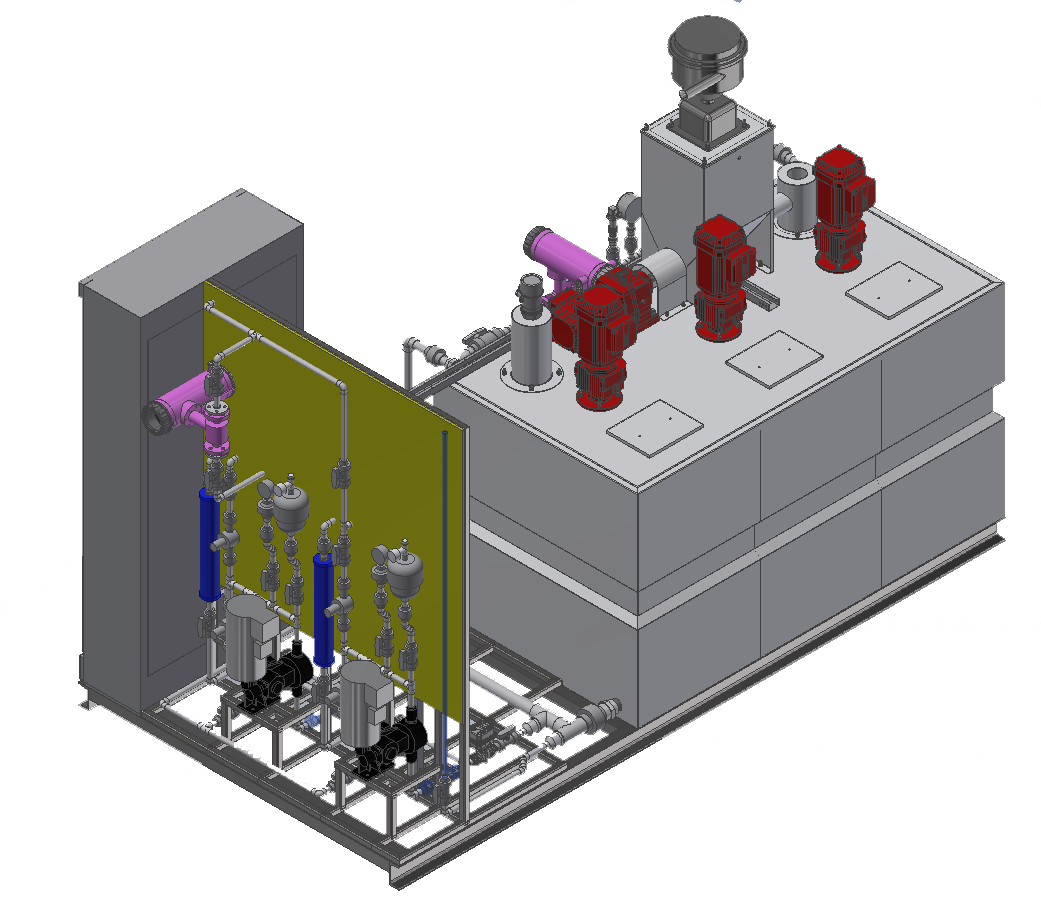
\includegraphics[height=10cm]{g0.PNG}
   \end{figure}
}
\date{}

\maketitle % 封面

\tableofcontents % 目录

\newpage % 换页

%\part{系统组成}
%ctex的\chapter{sdsg}是不能用的
\section{系统组成及功能说明}

   加药装置的主要组成部分,如下图\ref{fig:p1}或图\ref*{fig:p2}所示。
   \par也可以参考在线三维模型{\url{http://www.wuyumingtechnology.xyz/2022-Ningxia-Qingshuihe-KMnO4-M155/KMnO4.html}}。
   在线三维模型加载需要一定时间。
   \subsection{系统构成图}

      \begin{figure}[h]
         \centering

         \begin{tikzpicture}
            %定义图像
            \node at (0,0) {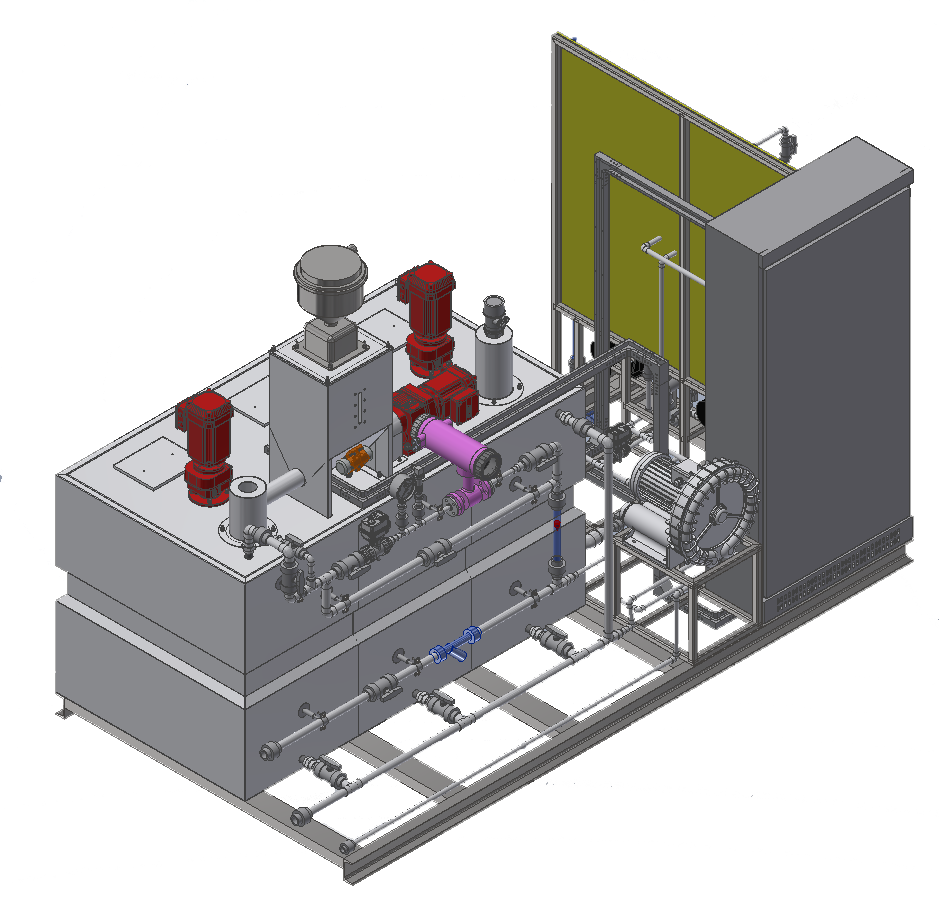
\includegraphics[height=15cm]{g01.PNG}};

            %说明
            \node at (7,-4) (1) [text_box] {进水电磁流量计};
            \draw [arrow] (1) -- (0,0);
            \node at (-7,-6) (2) [text_box] {进水口};
            \draw [arrow] (2) -- (-3.2,-5);
            \node at (-6,-7) (3) [text_box] {排液口};
            \draw [arrow] (3) -- (-2.8,-6.1);
            \node at (-4,-8) (4) [text_box] {加药口};
            \draw [arrow] (4) -- (-2,-6.5);
            \node at (4,-7) (5) [text_box] {放空阀};
            \draw [arrow] (5) -- (-0.5,-4.2);
            \node at (0,-7) (6) [text_box] {放空阀};
            \draw [arrow] (6) -- (-2.5,-5.3);
            \node at (2,-7) (7) [text_box] {进水阀};
            \draw [arrow] (7) -- (-1.5,-3.9);
            \node at (7.5,-3) (8) [text_box] {真空上料器风机};
            \draw [arrow] (8) -- (4.1,-1.1);
            \node at (5,-6) (9) [text_box] {Y型过滤器};
            \draw [arrow] (9) -- (-0.5,-3.2);
            \node at (6,-5) (10) [text_box] {放空阀};
            \draw [arrow] (10) -- (1.5,-3.1);
            \node at (-7,3) (12) [text_box] {振荡器};
            \draw [arrow] (12) -- (-1.8,-0.1);
            \node at (7,6) (13) [text_box] {控制电柜};
            \draw [arrow] (13) -- (6,2);
            \node at (-7,2) (14) [text_box] {搅拌机};
            \draw [arrow] (14) -- (-4.5,0.2);
            \node at (5,7) (15) [text_box] {超声波液位计};
            \draw [arrow] (15) -- (0.4,2.3);
            \node at (0,7) (16) [text_box] {搅拌机};
            \draw [arrow] (16) -- (-0.5,2.4);
            \node at (-3,6) (17) [text_box] {螺旋进料器};
            \draw [arrow] (17) -- (-0.5,1);
            \node at (-8,-5) (18) [text_box] {进水电动阀};
            \draw [arrow] (18) -- (-1.5,-1.3);
            \node at (-8,-2) (19) [text_box] {进水压力表};
            \draw [arrow] (19) -- (-1,-0.6);
            \node at (-5,5) (20) [text_box] {料斗};
            \draw [arrow] (20) -- (-2,1);
            \node at (-8,-0.5) (21) [text_box] {进水压力变送器};
            \draw [arrow] (21) -- (-0.9,-0.5);

			% 辅助线
            % \def \xLimit {8};
            % \def \yLimit {8};
            % 
			% 辅助线
            \draw (-\xLimit,-\yLimit) [help lines] grid (\xLimit,\yLimit);
            \foreach \x in {-\xLimit, ...,\xLimit}{
               \node [red] at (\x, \yLimit) {\x};
               \node [red] at (\x, -\yLimit) {\x};
               \node [red] at (\x, 0) {\x};
            }
            \foreach \y in {-\yLimit, ...,\yLimit}
                  \node [red] at (-\xLimit, \y) {\y};
            \foreach \y in {-\yLimit, ...,\yLimit}
                  \node [red] at (\xLimit, \y) {\y};
            \foreach \y in {-\yLimit, ...,\yLimit}
                  \node [red] at (0, \y) {\y};


         \end{tikzpicture}
         \caption{系统组成}\label{fig:p1}
      \end{figure}

\newpage % 换页

      \begin{figure}[h]
         \centering

         \begin{tikzpicture}
            %图片
            \node at (0,0) {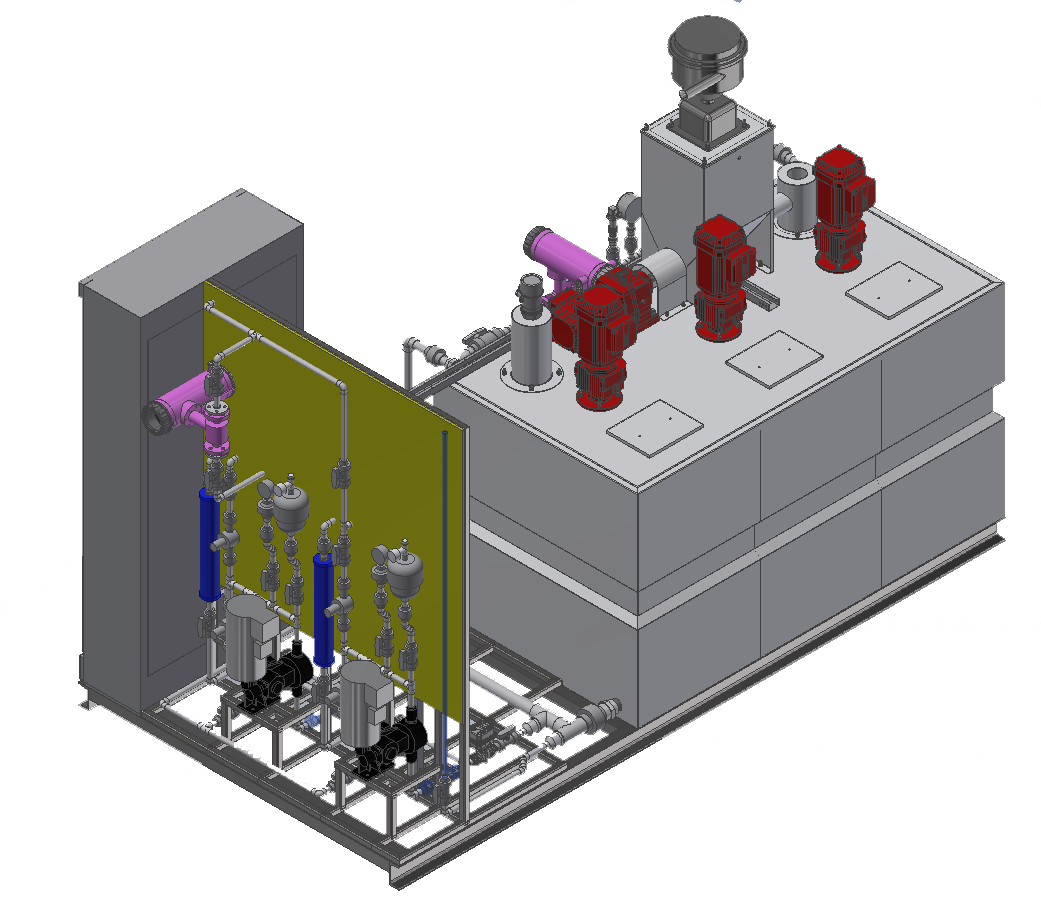
\includegraphics[height=12cm]{g0.PNG}};

            %说明
            \node at (7,5) (1) [text_box] {搅拌机};
            \draw [arrow] (1) -- (4.2,3.5);
            \node at (5,6) (2) [text_box] {料斗};
            \draw [arrow] (2) -- (3,3.5);
            \node at (7,-2) (3) [text_box] {搅拌机};
            \draw [arrow] (3) -- (2.5,2.3);
            \node at (6,-3) (4) [text_box] {搅拌机};
            \draw [arrow] (4) -- (1,1.5);
            \node at (-1,6) (5) [text_box] {进水压力变送器};
            \draw [arrow] (5) -- (1.3,3);
            \node at (1,7) (6) [text_box] {进水压力表};
            \draw [arrow] (6) -- (1.4,3.2);
            \node at (-3,4) (7) [text_box] {超声波液位计};
            \draw [arrow] (7) -- (0.1,2.2);
            \node at (-7,4) (8) [text_box] {电控柜};
            \draw [arrow] (8) -- (-5,2.5);
            \node at (-8,-2) (9) [text_box] {标定柱};
            \draw [arrow] (9) -- (-4.1,-1.6);
            \node at (-8,0) (9) [text_box] {背压阀};
            \draw [arrow] (9) -- (-3.9,-1.1);
            \node at (-8,-3) (10) [text_box] {安全阀/泄压阀};
            \draw [arrow] (10) -- (-4,-2.4);
            \node at (-7,-5) (11) [text_box] {计量泵};
            \draw [arrow] (11) -- (-3.7,-2.5);
            \node at (-2,5) (12) [text_box] {进水电磁流量计};
            \draw [arrow] (12) -- (0.5,2.5);
            \node at (-5,-6) (13) [text_box] {计量泵};
            \draw [arrow] (13) -- (-2.2,-3.5);
            \node at (-8,2) (14) [text_box] {加药电磁流量计};
            \draw [arrow] (14) -- (-4.5,0.6);
            \node at (0,-6) (15) [text_box] {阻尼器};
            \draw [arrow] (15) -- (-1.5,-1.6);
            \node at (-8,1) (16) [text_box] {隔膜压力表};
            \draw [arrow] (16) -- (-3.3,-0.5);
            \node at (3,-5) (17) [text_box] {可视液位计};
            \draw [arrow] (17) -- (-1,-1);

			% % 辅助线
         %    \def \xLimit {8};
         %    \def \yLimit {8};
         %    
			% 辅助线
            \draw (-\xLimit,-\yLimit) [help lines] grid (\xLimit,\yLimit);
            \foreach \x in {-\xLimit, ...,\xLimit}{
               \node [red] at (\x, \yLimit) {\x};
               \node [red] at (\x, -\yLimit) {\x};
               \node [red] at (\x, 0) {\x};
            }
            \foreach \y in {-\yLimit, ...,\yLimit}
                  \node [red] at (-\xLimit, \y) {\y};
            \foreach \y in {-\yLimit, ...,\yLimit}
                  \node [red] at (\xLimit, \y) {\y};
            \foreach \y in {-\yLimit, ...,\yLimit}
                  \node [red] at (0, \y) {\y};


         \end{tikzpicture}
         \caption{系统组成}\label{fig:p2}
      \end{figure}

   \subsection{系统功能说明}
      高锰酸钾自动制备投加装置主要分为自动制备系统和自动投加装置两部分组成。
      \par操作人员只需要设定好控制参数,系统将自动运行。
      \subsubsection{自动制备系统功能}
         自动制备系统将高锰酸钾固体粉料制备成溶液。
         \par主要设定参数:
         \begin{itemize}
            \item 溶液制备量。制备系统设计制备能力为1000L/h。
            \item 溶液浓度。常用浓度为1\% $\sim$ 2\%。
            \item 开机液位。储液池液位低于开机液位时,制备系统自动开机。
               客户可自行设置开机液位,
               出厂默认设置值为0.5米。
            \item 停机液位。储液池液位高于停机液位时,制备系统自动停机。
               客户可自行设置停机液位,
               出厂默认设置值为0.8米,
               设置值不可高于0.9米。
            \item 搅拌机间歇运行参数。
            搅拌机每运行若干分钟,
            则停止若干分钟,
            时长可设置。
            出厂默认设置值为每运行120分钟,
            则暂停5分钟。
            当系统处于溶液制备状态,
            螺旋进料器启动,
            进水电动阀打开时,
            搅拌机将持续运行,
            不会暂停。
            \item 进水低水压。
            进水压力低于此值制备系统自动停机,出厂设置值为2bar。
         \end{itemize}
         \par制备系统自动运行时,
         控制系统根据进水流量探头反馈,
         通过进水电动阀,
         将进水流量控制在上述设定的溶液制备量上。
         \par同时,控制系统根据上述设定参数,
         按以下公式\ref{powder-in}计算出螺旋进料器进料量(kg/h),
         控制进料器电机变频器,
         使进料量达到设定值。
         \begin{equation}
            \label{powder-in}
            \mbox{进料量}(kg/h) = \mbox{溶液制备量}(L/h)  \times \mbox{溶液浓度} (\%)
         \end{equation}
         \par制备系统料斗带有高、低料位报警探头,
         料斗料位过低进会自动停止溶液制备过程并发出报警。
         此时应使用真空上料机吸取高锰酸钾原料,
         物料足够时制备系统会恢复自动运行。

      \subsubsection{自动投加系统功能}
         自动投加系统按设定参数向进水总管投加高锰酸钾溶液。
         \par主要设定参数:
         \begin{itemize}
            \item 溶液投率。设计溶液投率为1mg/L,可修改。
            \item 溶液浓度。常用浓度为1\% $\sim$2\%。
            \item 源水低水量报警。
            源水水量低于此设定则自动停泵。
            \item 计量泵轮换设置。
            计量泵连续运行若干小时,
            则切换到另1台计量泵运行。
            \item 储液池低液位报警设置。
            低于此液位高锰酸钾溶液不足,
            自动停泵。
         \end{itemize}
         \par控制系统按以下公式\ref{chemical-flow}计算的流量,
         控制计量泵变频器,
         向进水总管投加制备好的高锰酸钾溶液。
         \begin{equation}
            \label{chemical-flow}
            \mbox{投加流量}(L/h) = \mbox{溶液投率}(mg/L) \times 
            \mbox{源水水量}(m^3/h) \div 
            \mbox{溶液浓度}(\%)
         \end{equation}


\newpage % 换页

\section{设备启动前准备}\label{sec:sg1}
   \subsection{紧固件检查}
      系统启动前,要先对所有的紧固件进行检查。
      紧固件包括底座固定螺栓、泵固定螺栓、马达连接螺栓以及所有的法兰连接螺栓等。
      如有松动情况,请将其上紧,如有脱落等情况,请按相应的规格补充相关的螺栓。

   \subsection{管道连接检查}
      检查管道中所有活接接头连接,如有松脱情况需要重新上紧。

   \subsection{检查系统中各阀门状态}
      \subsubsection{各检修阀门应处于关闭状态}\label{sec:sg3}
         检修阀门包括检修排液阀、
         检修旁通阀、放空阀等,
         正常运行时均应处于关闭状态。
      \begin{figure}[h]
         \centering
         \begin{tikzpicture}
            %图片
            \node at (0,0) {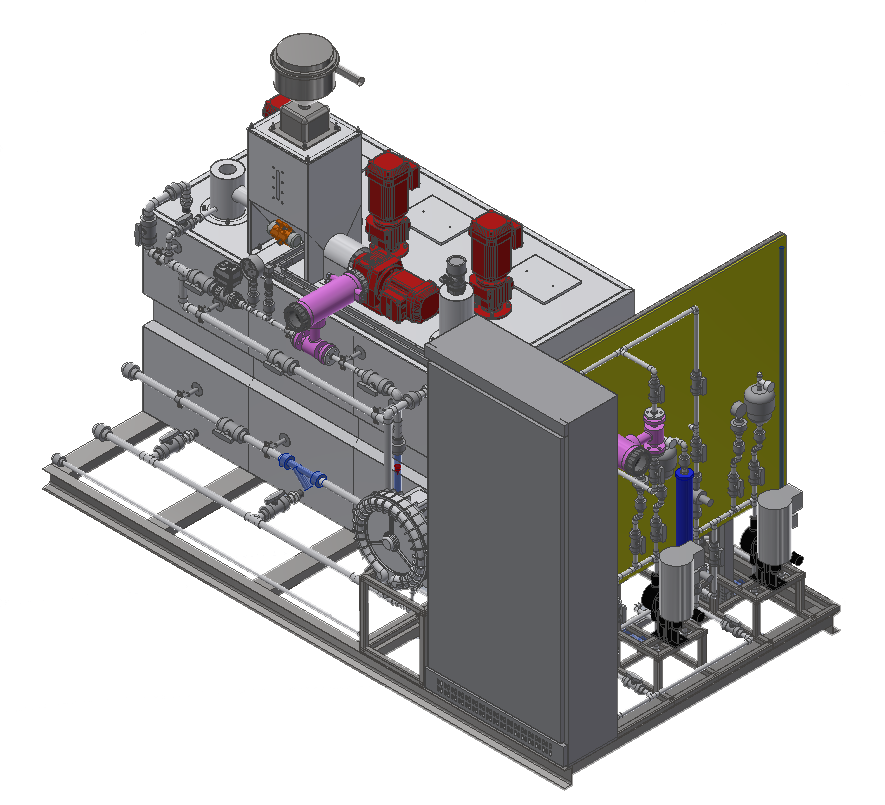
\includegraphics[height=13cm]{g02.PNG}};

            %说明
            \def \itemNumber {1};
            \def \centertPoint {4.4, -2.5};
            \node at (7,-5) (\itemNumber) [text_box] {检修排液阀};
            \draw [arrow] (\itemNumber) -- (\centertPoint);
            \draw (\centertPoint) circle (0.5)[red];
            \def \itemNumber {2};
            \def \centertPoint {4.1,0.2};
            \node at (6,4) (\itemNumber) [text_box] {检修旁通阀};
            \draw [arrow] (\itemNumber) -- (\centertPoint);
            \draw (\centertPoint) circle (0.5)[red];
            \def \itemNumber {3};
            \def \centertPoint {-2.6,0.7};
            \node at (-7,4) (\itemNumber) [text_box] {检修旁通阀};
            \draw [arrow] (\itemNumber) -- (\centertPoint);
            \draw (\centertPoint) circle (0.5)[red];
            \def \itemNumber {4};
            \def \centertPoint {-4.3, -0.7};
            \node at (-7,-3) (\itemNumber) [text_box] {放空阀};
            \draw [arrow] (\itemNumber) -- (\centertPoint);
            \draw (\centertPoint) circle (0.5)[red];
            \def \itemNumber {5};
            \def \centertPoint {-2.7,-1.7};
            \node at (-5,-4) (\itemNumber) [text_box] {放空阀};
            \draw [arrow] (\itemNumber) -- (\centertPoint);
            \draw (\centertPoint) circle (0.5)[red];

			% 辅助线
            \def \xLimit {8};
            \def \yLimit {6};
            % 
			% 辅助线
            \draw (-\xLimit,-\yLimit) [help lines] grid (\xLimit,\yLimit);
            \foreach \x in {-\xLimit, ...,\xLimit}{
               \node [red] at (\x, \yLimit) {\x};
               \node [red] at (\x, -\yLimit) {\x};
               \node [red] at (\x, 0) {\x};
            }
            \foreach \y in {-\yLimit, ...,\yLimit}
                  \node [red] at (-\xLimit, \y) {\y};
            \foreach \y in {-\yLimit, ...,\yLimit}
                  \node [red] at (\xLimit, \y) {\y};
            \foreach \y in {-\yLimit, ...,\yLimit}
                  \node [red] at (0, \y) {\y};


         \end{tikzpicture}
         \caption{各检修阀位置}\label{fig:p3}
      \end{figure}

\newpage

      \par上图\ref{fig:p3}所示为
      检修排液阀、
      检修旁通阀、
      放空阀等阀门所在位置。
      % \par表示这是一段,新开一段才会自动退2个空格
      \par检修排液阀的作用,
      用于在检修时释放系统压力,
      避免管道内化学品喷射出来。
      \par检修旁通阀的作用,
      是电磁流量计、电动阀、压力变送器、压力表等需要检修时,
      关闭其上下游阀门,
      打开检修旁通阀,
      可在手动状态维持系统运行。
      放空阀的作用,
      在于检修制备槽、熟化槽、储药槽时,
      或长期存放装置暂不使用时,
      将槽内积液排空。
      \par正常工作时应将检修排液阀、检修旁通阀关闭。

      \subsubsection{标定柱控制阀应处于关闭状态}
      \begin{figure}[h]
         \centering
         \begin{tikzpicture}
            %图片
            \node at (0,0) {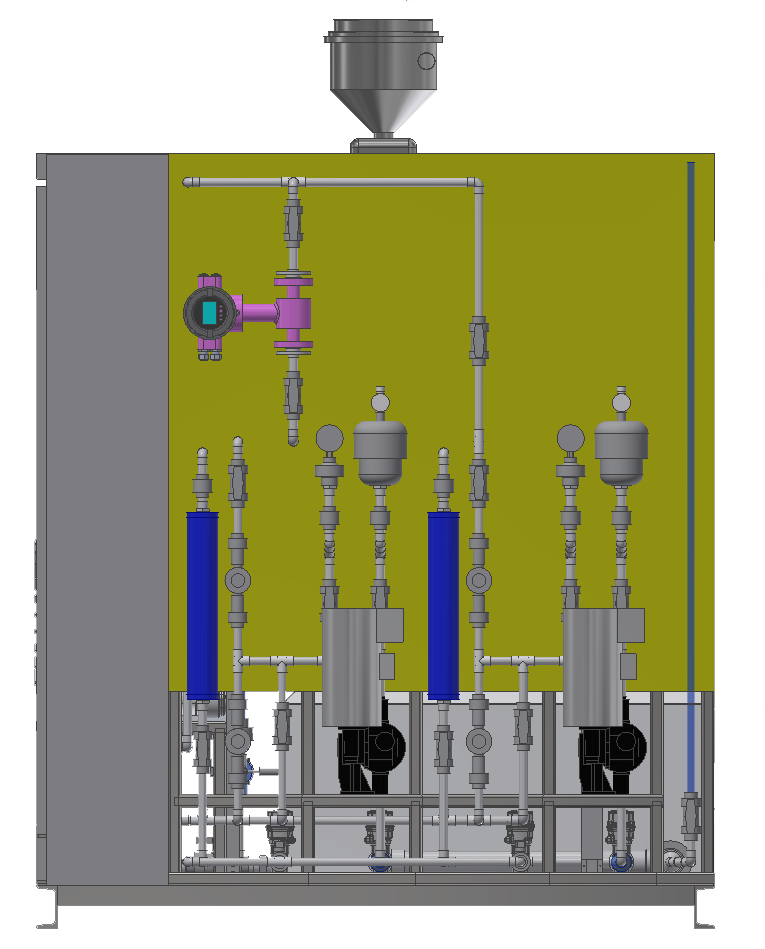
\includegraphics[height=12cm]{g05.PNG}};

            %说明
            \def \itemNumber {1};
            \def \centertPoint {0.7, -3.4};
            \node at (6,-5) (\itemNumber) [text_box] {标定柱控制阀};
            \draw [arrow] (\itemNumber) -- (\centertPoint);
            \draw (\centertPoint) circle (0.5)[red];
            \def \itemNumber {2};
            \def \centertPoint {-2.3, -3.4};
            \node at (-6,-5) (\itemNumber) [text_box] {标定柱控制阀};
            \draw [arrow] (\itemNumber) -- (\centertPoint);
            \draw (\centertPoint) circle (0.5)[red];

			% 辅助线
            \def \xLimit {8};
            \def \yLimit {7};
            % 
			% 辅助线
            \draw (-\xLimit,-\yLimit) [help lines] grid (\xLimit,\yLimit);
            \foreach \x in {-\xLimit, ...,\xLimit}{
               \node [red] at (\x, \yLimit) {\x};
               \node [red] at (\x, -\yLimit) {\x};
               \node [red] at (\x, 0) {\x};
            }
            \foreach \y in {-\yLimit, ...,\yLimit}
                  \node [red] at (-\xLimit, \y) {\y};
            \foreach \y in {-\yLimit, ...,\yLimit}
                  \node [red] at (\xLimit, \y) {\y};
            \foreach \y in {-\yLimit, ...,\yLimit}
                  \node [red] at (0, \y) {\y};


         \end{tikzpicture}
         \caption{标定柱控制阀位置}\label{fig:p4}
      \end{figure}

      上图\ref{fig:p4}所示为标定柱控制阀所在位置。
      图中标定柱控制阀为打开状态,系统启动前应将其关闭。
      \par标定柱的作用是校正流量监控仪表以及确定计量泵真实流量,
      进行流量标定时应将标定柱控制阀,正常工作时应将其关闭。\\

\subsubsection{其余阀门均处于开启状态}
      除上述特别说明之外的所有阀门,在正常工作状态下,都应处于开启状态。

\newpage % 换页

\section{日常操作}
   \subsection{制备投加系统上电}
      \subsubsection{上电前检查}
         上电之前,
         应先确认电柜电源进线有电,
         且没有缺相。

      \begin{figure}[h]
         \centering
         \begin{tikzpicture}
            %图片
            \node at (0,0) {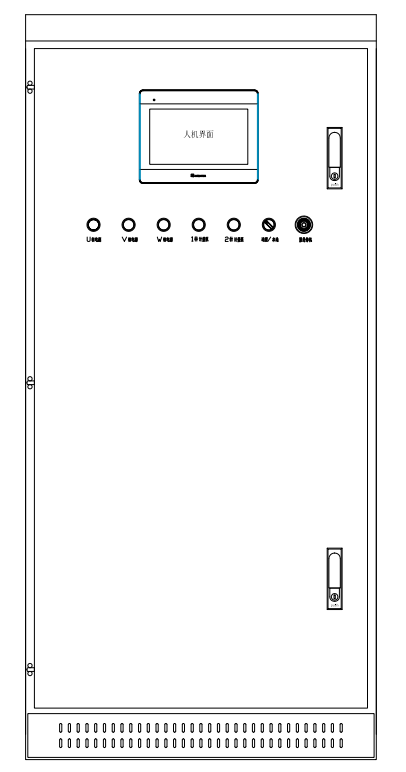
\includegraphics[height=10cm]{g03.PNG}};

            %说明
            \def \itemNumber {1};
            \def \centertPoint {-1.6, 1.8};
            \node at (-1,1.5) (\itemNumber) [text_box] {电柜电源进线指示灯};
            \draw (\centertPoint) rectangle +(1.3,0.5)[red];

			% 辅助线
            \def \xLimit {8};
            \def \yLimit {7};
            % 
			% 辅助线
            \draw (-\xLimit,-\yLimit) [help lines] grid (\xLimit,\yLimit);
            \foreach \x in {-\xLimit, ...,\xLimit}{
               \node [red] at (\x, \yLimit) {\x};
               \node [red] at (\x, -\yLimit) {\x};
               \node [red] at (\x, 0) {\x};
            }
            \foreach \y in {-\yLimit, ...,\yLimit}
                  \node [red] at (-\xLimit, \y) {\y};
            \foreach \y in {-\yLimit, ...,\yLimit}
                  \node [red] at (\xLimit, \y) {\y};
            \foreach \y in {-\yLimit, ...,\yLimit}
                  \node [red] at (0, \y) {\y};


         \end{tikzpicture}
         \caption{电柜操作面板布局}\label{fig:p5}
      \end{figure}

      \par如上图\ref*{fig:p5}所示,
      3个电源指示灯全亮,
      即表示电源进线有电,
      且没有缺相,
      这时可以给电柜上电。

      \newpage % 换页

      \subsubsection{电柜上电}
         \begin{figure}[h]
            \centering
            \begin{tikzpicture}
               %图片
               \node at (0,0) {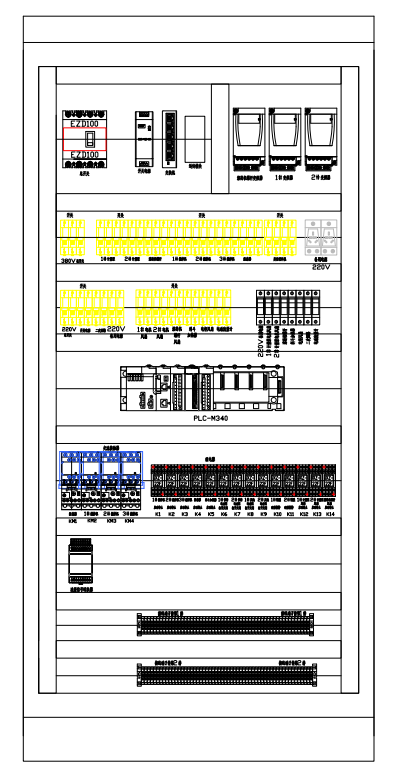
\includegraphics[height=10cm]{g04.PNG}};

               %说明
               \def \itemNumber {1};
               \def \centertPoint {-1.9, 2.7};
               \node at (-3,3) (\itemNumber) [text_box] {电柜总开关};
               \draw (\centertPoint) rectangle +(0.8,0.9)[red];
               \def \itemNumber {2};
               \def \centertPoint {-1.9, 1.5};
               \node at (-3,2) (\itemNumber) [text_box] {其余开关};
               \draw (\centertPoint) rectangle +(3.2,0.7)[red];
               \def \itemNumber {3};
               \def \centertPoint {-1.9, 0.6};
               \node at (-3,1) (\itemNumber) [text_box] {其余开关};
               \draw (\centertPoint) rectangle +(2.4,0.7)[red];

            % 辅助线
               \def \xLimit {8};
               \def \yLimit {7};
            %    
			% 辅助线
            \draw (-\xLimit,-\yLimit) [help lines] grid (\xLimit,\yLimit);
            \foreach \x in {-\xLimit, ...,\xLimit}{
               \node [red] at (\x, \yLimit) {\x};
               \node [red] at (\x, -\yLimit) {\x};
               \node [red] at (\x, 0) {\x};
            }
            \foreach \y in {-\yLimit, ...,\yLimit}
                  \node [red] at (-\xLimit, \y) {\y};
            \foreach \y in {-\yLimit, ...,\yLimit}
                  \node [red] at (\xLimit, \y) {\y};
            \foreach \y in {-\yLimit, ...,\yLimit}
                  \node [red] at (0, \y) {\y};


            \end{tikzpicture}
            \caption{电柜内布局}\label{fig:p6}
         \end{figure}

      \par电柜内布局如上图\ref*{fig:p6}所示。
      \par依次打开
      电柜总开关、380V总开关、220V总开关、开关电源开关、
      二次回路开关,
      以及
      1号计量泵、
      2号计量泵、
      溶药机螺杆、
      1号搅拌机、
      2号搅拌机、
      3号搅拌机、
      真空上料机等380V用电设备开关,
      和1号计量泵电机独立冷却风扇、
      2号计量泵电机独立冷却风扇、
      溶药机螺杆独立冷却风扇、
      电柜风扇、
      电磁流量计等220V用电设备开关。

      \par其中,振荡器和料斗加热器开关不需要打开。
      振荡器和料斗加热器,
      是在原料比较潮湿,
      并且已经有板结的情况下使用,
      正常情况下不需要使用,
      所以正常情况下不用打开。

      \subsubsection{观察加药装置各系统状态}
      观察人机界面、变频器、PLC及流量仪表工作状态是否正常。
      在正常情况下,人机界面、变频器及流量仪表显示器均应该点亮,PLC上应无红灯闪烁。

      \subsubsection{异常情况处理}
      加药系统上电如发现异常情况,请与加药系统售后服务人员联系。
      如需自行处理,请先详细查阅附件技术资料,自行处理若操作不当,有可能导致加药系统损坏。

         \newpage % 换页

   \subsection{主控制界面}\label{sec:s1}
      自动制备投加系统主要通过人机界面设定系统运行参数。
      \par人机界面的主控制界面如下图\ref{fig:g7}所示。
      \par主控制界面可以切换到其他控制界面,
      下图\ref{fig:g7}红圈内为切换到其他控制界面的区域。
      \par同时,主控制界面设置高锰酸钾投加系统的运行参数。

      \begin{figure}[h]
         \centering
            \begin{tikzpicture}
               % \draw (-8,-4) [help lines] grid (8,4);
               % \draw [red] (-8,0) -- (8,0);
               % \draw [red] (0,-4) -- (0,4);
               %图片
               \node at (0,0) {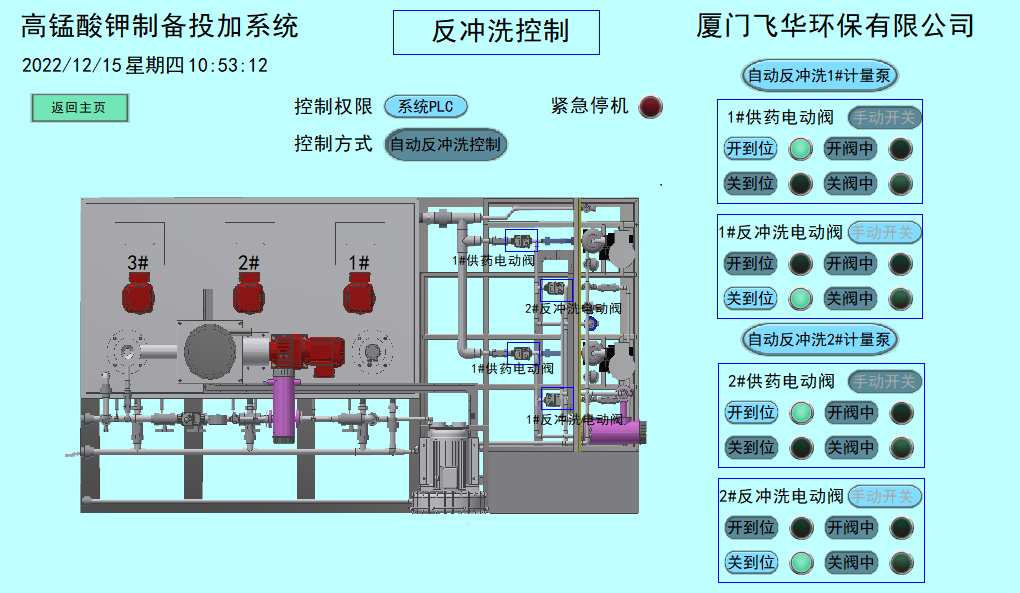
\includegraphics[height=8cm]{g6.PNG}};

               %说明
               \node at (-2,3) (1) [text_box, color=red] {界面切换区域};
               % \draw [arrow] (1) -- (-3,6);
               \draw (-6.8,0.5) rectangle +(5,2.2)[red];
            \end{tikzpicture}
         \caption{主控制界面}\label{fig:g7}
      \end{figure}

   \subsection{设置制备系统参数}\label{sec:sg5}
      制备系统开始运行前,
      要先设置好制备系统运行参数。
      \par在上图\ref{fig:g7}主控制界面上,
      按”溶液制备“按钮,
      切换到溶液制备控制界面。
      \par或者按”搅拌机控制“按钮,
      切换到搅拌机控制界面。
      \par制备系统运行参数设置好之后,
      将会自动运行,
      无须人工参与。
      出现供水水压过低,
      或料斗料位过低,
      制备系统将自动停机。

      \newpage

      \begin{figure}[h]
         \centering
            \begin{tikzpicture}
               % \draw (-8,-4) [help lines] grid (8,4);
               % \draw [red] (-8,0) -- (8,0);
               % \draw [red] (0,-4) -- (0,4);
               %图片
               \node at (0,0) {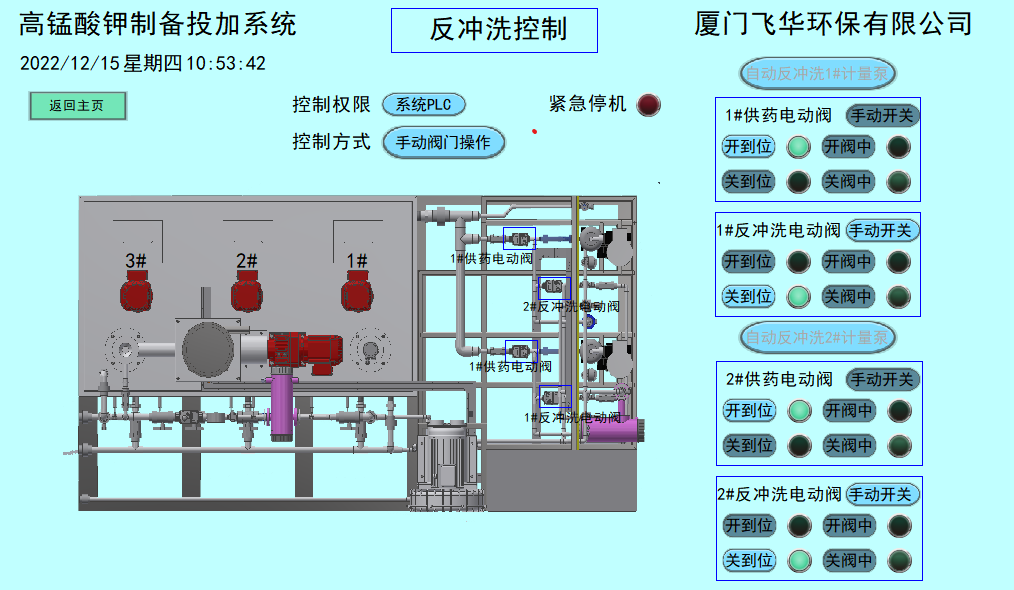
\includegraphics[height=8cm]{g7.PNG}};

               %说明
               \node at (-1,3) (1) [text_box, color=red] {切换到搅拌机控制};
               \draw [arrow, color=red] (1) -- (-4,2.5);
               \node at (-4,2) (1) [text_box, color=red] {参数1};
               \node at (5.9,2.6) (1) [text_box, color=red] {参数2};
               \node at (5.9,-0.9) (1) [text_box, color=red] {参数3};
            \end{tikzpicture}
         \caption{溶液制备控制界面}\label{fig:g8}
            \begin{tikzpicture}
               % \draw (-8,-4) [help lines] grid (8,4);
               % \draw [red] (-8,0) -- (8,0);
               % \draw [red] (0,-4) -- (0,4);
               %图片
               \node at (0,0) {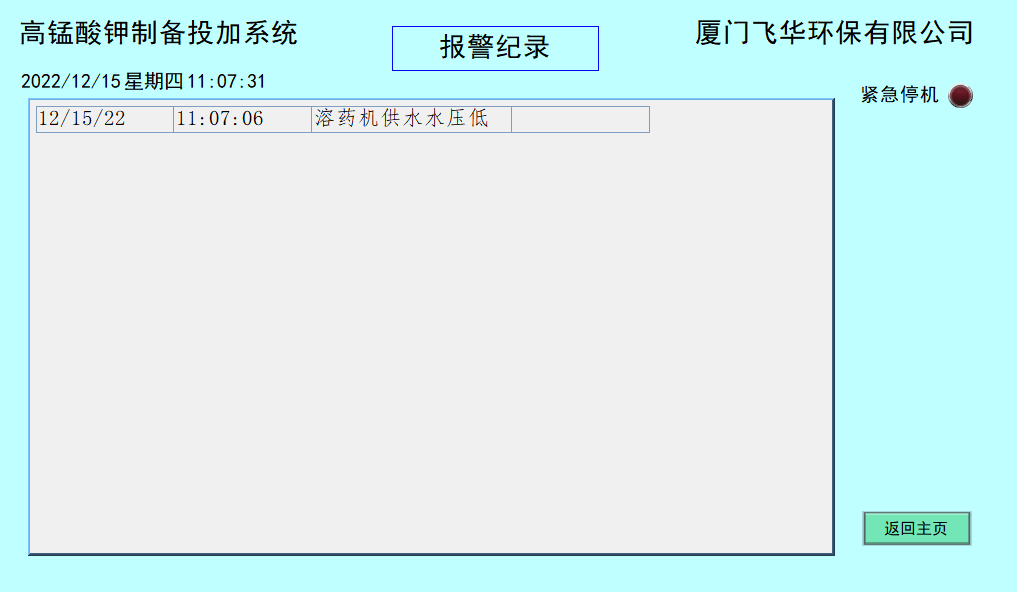
\includegraphics[height=8cm]{g8.PNG}};

               %说明
               \node at (-2,3) (1) [text_box, color=red] {切换到溶液制备};
               \draw [arrow, color=red] (1) -- (-4,2.5);
               \node at (-4.5,-0.5) (1) [text_box, color=red] {参数4};
            \end{tikzpicture}
         \caption{搅拌机控制界面}\label{fig:g9}
      \end{figure}

      \par在上图\ref{fig:g8}以及图\ref{fig:g9}界面设置好以下参数:
      \begin{enumerate}
         \item 制备系数。
            \begin{itemize}
               \item 溶液制备量。制备系统设计制备能力为1000L/h。
               \item 高锰酸钾浓度。常用浓度为1\% -- 2\%,默认设置为1\%。
               \item 溶液密度。以1\%浓度算,溶液密度为1.006g/cm$^{3}$。
            \end{itemize}
         \item 开机、停机液位。
            \begin{itemize}
               \item 开机液位。储液池液位低于开机液位时,制备系统自动开机,默认0.5m。
               \item 停机液位。储液池液位高于停机液位时,制备系统自动停机,默认0.9m。
            \end{itemize}
         \item 低水压停机值。进水压力低于此值制备系统自动停机,出厂设置值为2bar。
         \item 搅拌机间歇运行参数。搅拌机每运行若干分钟,则停止若干分钟。
            \begin{itemize}
               \item 运行时长。默认30min。
               \item 间歇时长。默认5min。
            \end{itemize}
      \end{enumerate}
      

   \subsection{制备系统供水、上料}
      \subsubsection{制备系统供水}\label{sec:sg2}
         连接制备系统供水管道,
         确认供水压力高于低水压停机值(出厂设定为2bar)。
         如果供水压力低于低水压停机值,
         制备系统会自动停机。
      \begin{figure}[h]
         \centering
            \begin{tikzpicture}
               % \draw (-8,-4) [help lines] grid (8,4);
               % \draw [red] (-8,0) -- (8,0);
               % \draw [red] (0,-4) -- (0,4);
               %图片
               \node at (0,0) {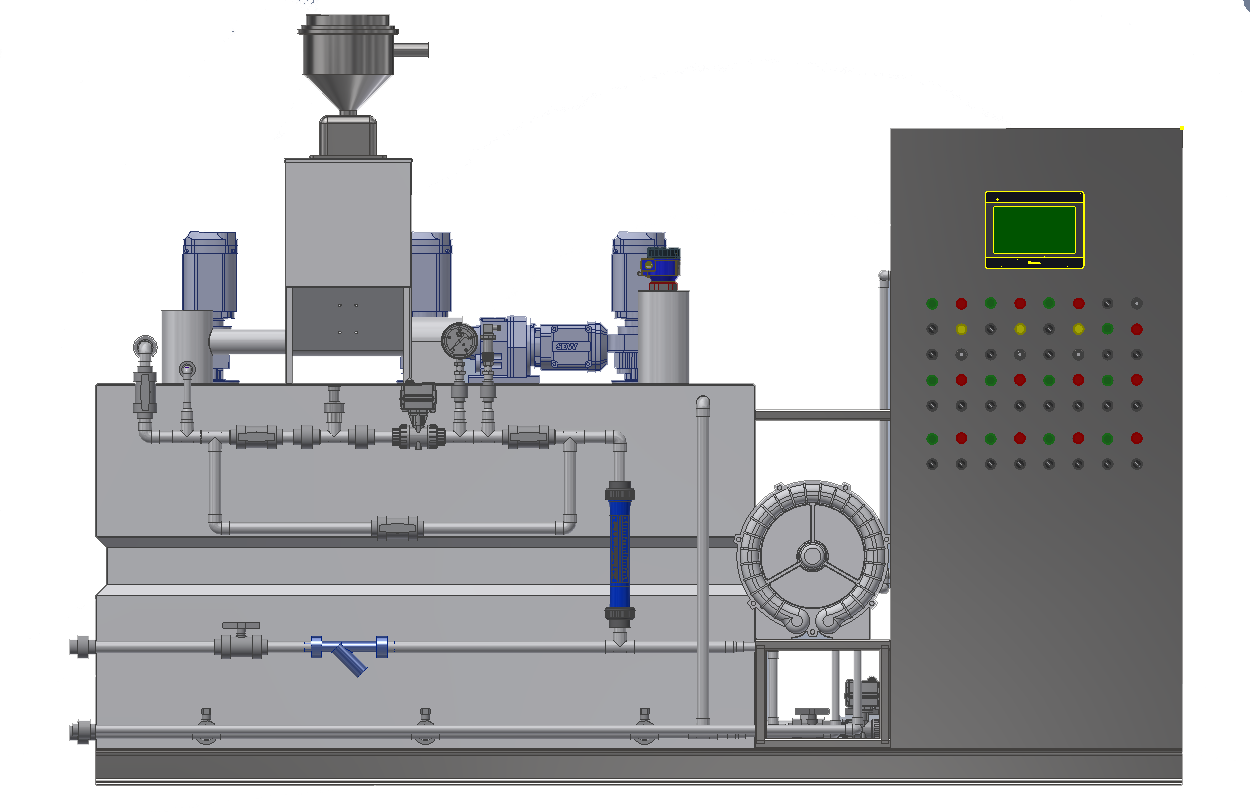
\includegraphics[height=8cm]{g9.PNG}};

               %说明
               \node at (-8,-3) (1) [text_box] {进水管};
               \draw [arrow] (1) -- (-5.2,-2.3);
               \draw (-5.2,-2.3) circle (0.5)[red];
               \node at (4,4) (2) [text_box] {进水压力表及压力变送器};
               \draw [arrow] (2) -- (-1.5,0.5);
               \draw (-1.5,0.5) circle (0.5)[red];
               \node at (-6,3) (3) [text_box] {进水流量探头};
               \draw [arrow] (3) -- (-2.8,0);
               \draw (-2.8,0) circle (0.5)[red];
               \node at (7,-3) (4) [text_box] {转子流量计};
               \draw [arrow] (4) -- (0,-1.5);
               \draw (0,-1.5) circle (0.5)[red];
               \node at (7,2) (5) [text_box] {真空上料机};
               \draw [arrow] (5) -- (2,-1.5);
               % \draw (2,-1.5) circle (0.5)[red];
            \end{tikzpicture}
         \caption{制备系统供水说明}\label{fig:g10}
      \end{figure}

      \subsubsection{制备系统上料}
         制备系统正常运行,
         需要保证料斗内有足够高锰酸钾粉料,
         料斗内有物位探头,
         料位过低,
         制备系统则自动停机。
         \par料斗内原料不足时,
         应使用真空上料机(参考\ref{sec:sg2}的图\ref{fig:g10}),
         向料斗内补充原料。

         \par启动真空上料机操作流程如下:
         \begin{enumerate}
            \item 打开真空上料机电源开关。见下图\ref{fig:g11}。
            \item 将吸料嘴伸入高锰酸钾粉料包装内。见下图\ref{fig:g11}。
            \item 按run/stop按钮启动真空上料机。
            启动真空上料机之后,
            上料机会自动运行/停止/运行间歇运行,
            方便已经吸上的粉料落入料斗内,
            过程中无须人工干预。见下图\ref{fig:g11}。
            \item 上料过程中应通过人机界面观察料斗内料位状态。见下图\ref{fig:g12}。
         \end{enumerate}

         \begin{figure}[h]
            \centering
               \begin{tikzpicture}
                  % \draw (-8,-4) [help lines] grid (8,4);
                  % \draw [red] (-8,0) -- (8,0);
                  % \draw [red] (0,-4) -- (0,4);
                  %图片
                  \node [rotate=-90] at (0,0) {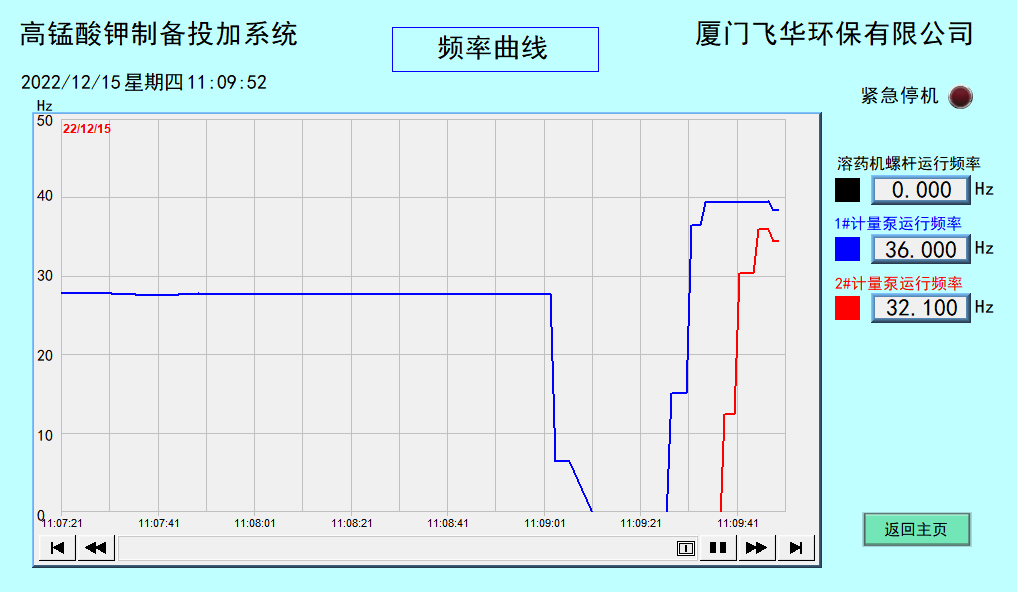
\includegraphics[height=6.6cm]{g10.PNG}};

                  %说明
                  \node at (-6,-2) (1) [text_box] {吸料嘴};
                  \draw [arrow] (1) -- (-2,0.7);
                  \draw (-2,0.7) circle (0.5)[red];
                  \node at (6,-2) (4) [text_box] {run/stop按钮};
                  \draw [arrow] (4) -- (-0.4,0.4);
                  \draw (-0.4,0.4) circle (0.3)[red];
                  \node at (6,3) (5) [text_box] {电源开关};
                  \draw [arrow] (5) -- (1.5,1);
                  \draw (1.5,1) circle (0.8)[red];
               \end{tikzpicture}
            \caption{真空上料机结构说明}\label{fig:g11}
         % \end{figure}

         % \begin{figure}[h]
         %    \centering
               \begin{tikzpicture}
                  % \draw (-8,-4) [help lines] grid (8,5);
                  % \draw [red] (-8,0) -- (8,0);
                  % \draw [red] (0,-4) -- (0,4);
                  %图片
                  \node at (0,0) {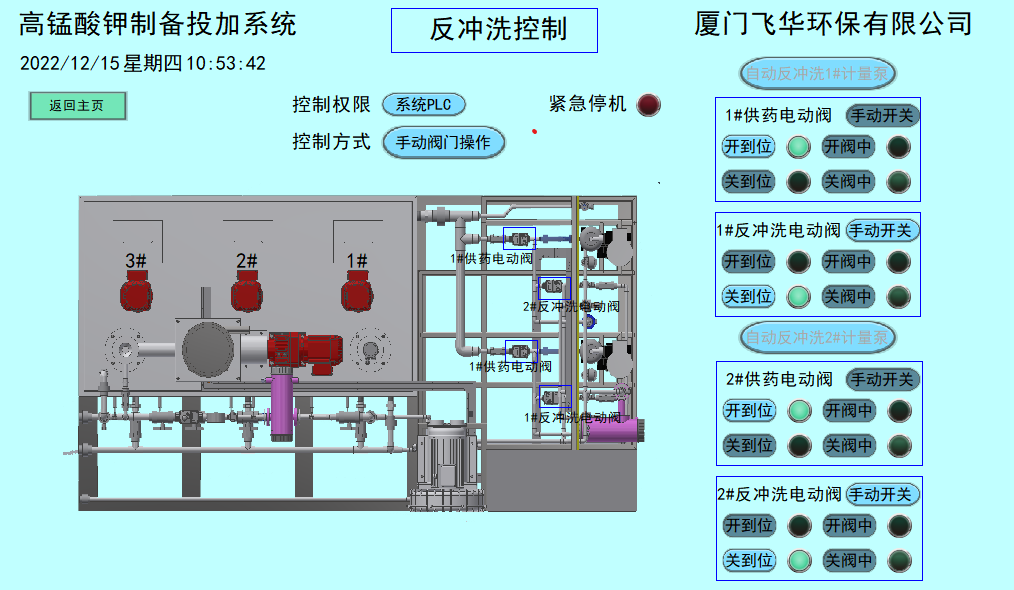
\includegraphics[height=8cm]{g7.PNG}};

                  %说明
                  \node at (-2.5,2) (1) [text_box, color=red] {料斗料位};
                  \draw [arrow, color=red] (1) -- (-5,-0.2);
                  \draw (-6.8,-0.9) rectangle +(3.3,1.2)[red];
               \end{tikzpicture}
            \caption{溶液制备控制界面}\label{fig:g12}
         \end{figure}

         \newpage

            已经吸入足够粉料,或料斗料位探头高报警,则应停止真空上料机。见上图\ref{fig:g12}。
         \par停止真空上料机操作流程如下:
         \begin{enumerate}
            \item 按run/stop按钮启动真空上料机。见上图\ref{fig:g11}。
            \item 将吸料嘴伸入高锰酸钾粉料包装内。见上图\ref{fig:g11}。
            \item 打开真空上料机电源开关。见上图\ref{fig:g11}。
         \end{enumerate}

   \subsection{设置投加系统参数}
        投加系统运行参数设置好之后,
        系统将会自动按相应参数向进水总管投加高锰酸钾,
        无须人工参与。
        \par源水流量过低,
        或储液池液位过低,
        制备系统将自动停机。

        \begin{figure}[h]
            \centering
                \begin{tikzpicture}
                %图片
                \node at (0,0) {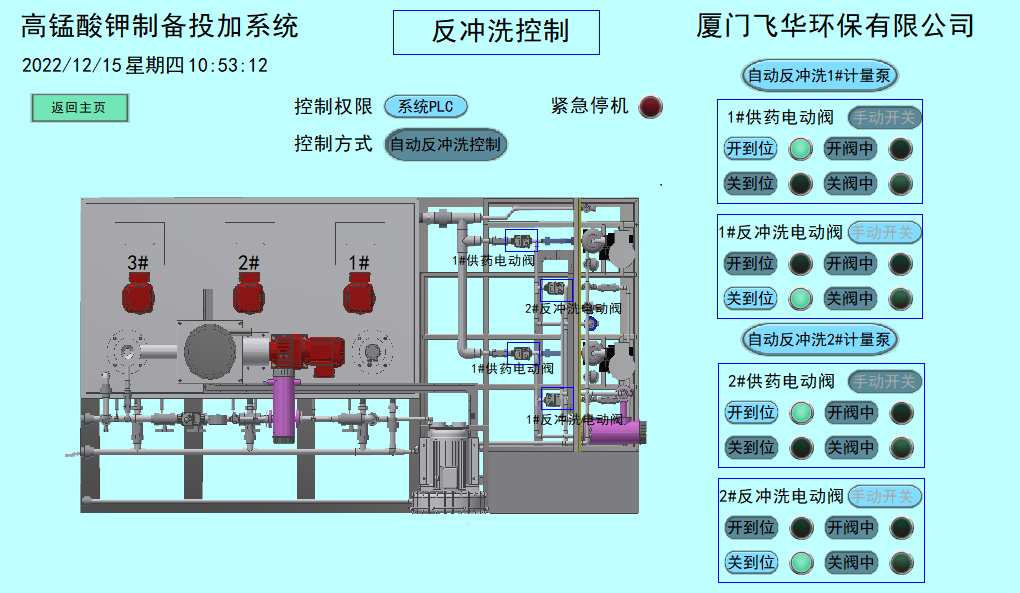
\includegraphics[height=8cm]{g6.PNG}};

                %说明
                \node at (-4.2,0.2) (1) [text_box, color=red] {参数1};
                \node at (4.3,2.3) (2) [text_box, color=red] {参数2};
                \node at (5.5,0.6) (3) [text_box, color=red] {参数2};
                \node at (-2.2,-3.6) (4) [text_box, color=red] {参数3};
                \node at (5.4,-1.8) (5) [text_box, color=red] {参数4};
                \node at (-5.2,-1.8) (6) [text_box, color=red] {参数4};

                %坐标辅助线
                % \draw (-8,-4) [help lines] grid (8,4);
                % \draw [red] (-8,0) -- (8,0);
                % \draw [red] (0,-4) -- (0,4);
                \end{tikzpicture}
            \caption{成品投加控制界面}\label{fig:g13}
        \end{figure}

      \par在上图\ref{fig:g13}界面设置以下参数:
      \begin{enumerate}
         \item 投加系数。
            \begin{itemize}
                \item 溶液投率。设计溶液投率为1mg/L即每L源水投加1mg高锰酸钾固体。
                \item 溶液密度。以1\%浓度算,溶液密度为1.006g/cm$^{3}$。
                \item 高锰酸钾浓度。在溶液制备参数中已设置(见\ref{sec:sg5}第\pageref{sec:sg5}页),此处无须再设置。
            \end{itemize}
         \item 停泵条件。
            \begin{itemize}
               \item 源水低流量。源水流量过低,投加系统自动停泵,默认5m$^{3}$/h。
               \item 储液池低液位。储液池液位过低时,投加系统自动停泵,默认0.2m。
            \end{itemize}
        \item 计量泵轮换设置。计量泵连续运行若干小时,则切换到另1台计量泵运行,默认8小时。
        \item 计量泵冲程长度。计量泵当前冲程长度,默认是60\%,如要修改请参考计量泵操作说明。
      \end{enumerate}

    \subsection{累积记录、报警记录、运行曲线、历史数据}
        高锰酸钾自动制备投加系统运行状态监控界面有累积记录、报警记录、运行曲线等、历史数据。
        \par上述几个界面,
        均可从主控制界面进入,
        参考\ref{sec:sg1}第\pageref{sec:sg1}页图\ref{fig:g7}。

        \subsubsection{累积记录}
            \begin{figure}[h]
                \centering
                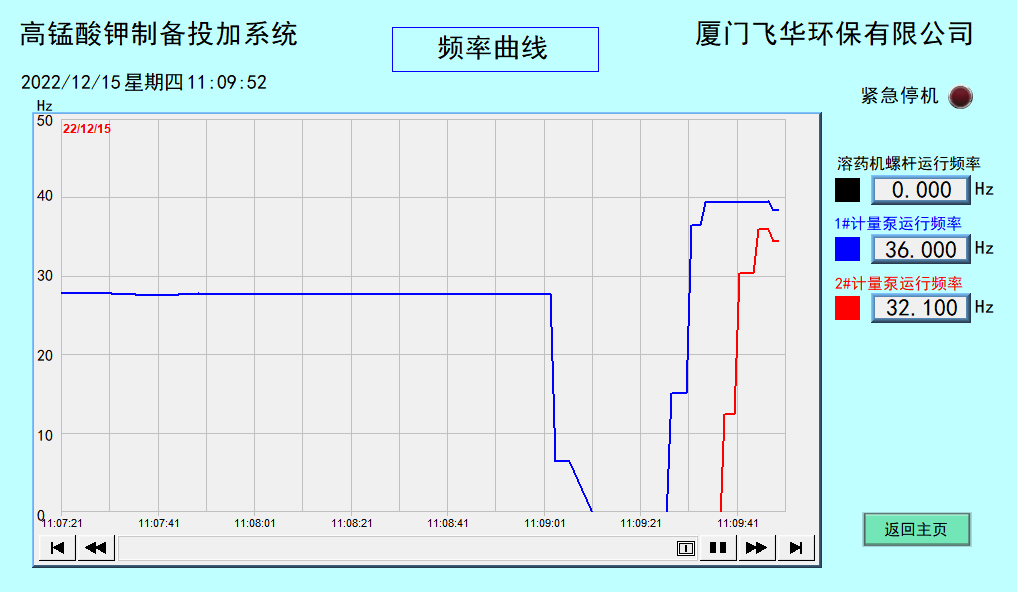
\includegraphics[height=6cm]{g10.PNG}
                \caption{累积纪录}\label{fig:g14}
            \end{figure}
            
        \subsubsection{报警记录}
            \begin{figure}[h]
                \centering
                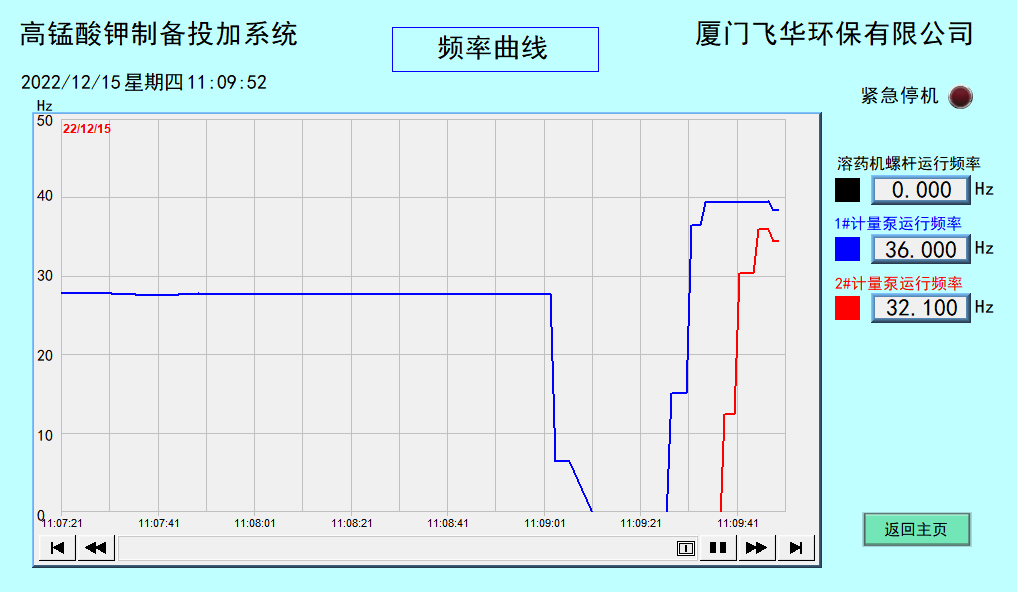
\includegraphics[height=6cm]{g10.PNG}
                \caption{报警记录}\label{fig:g15}
            \end{figure}

        \newpage

        \subsubsection{运行曲线}
            \begin{figure}[h]
                \centering
                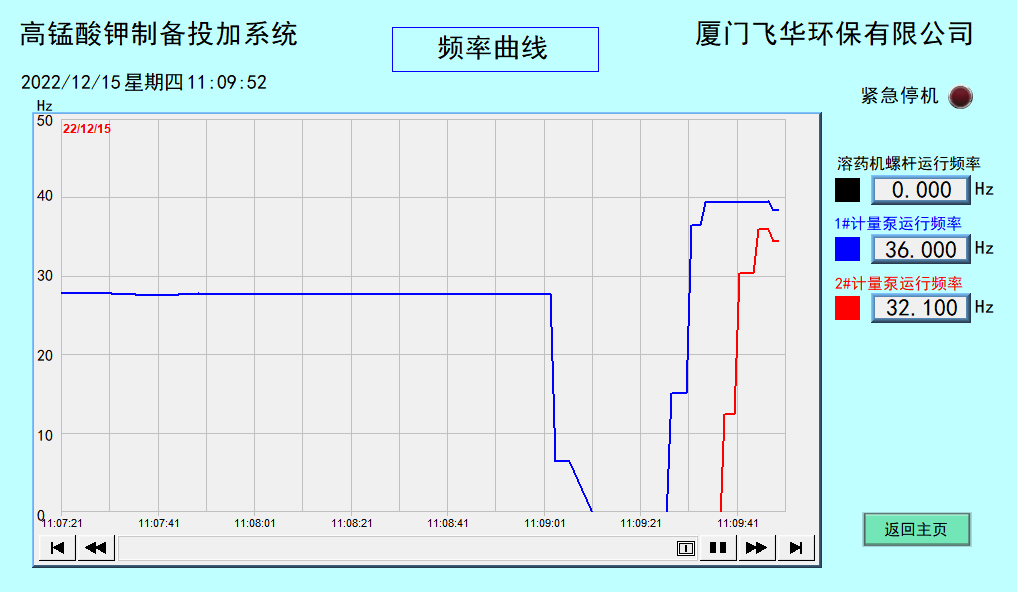
\includegraphics[height=6cm]{g10.PNG}
                \caption{加药流量曲线}\label{fig:g16}
               \quad\\ 
                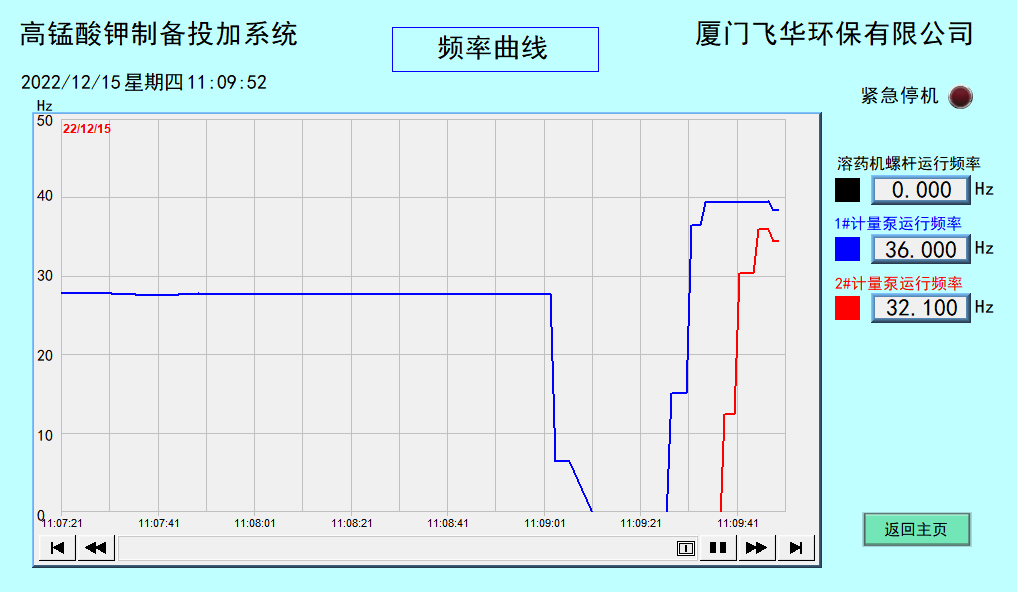
\includegraphics[height=6cm]{g10.PNG}
                \caption{电机频率曲线}\label{fig:g17}
            \end{figure}

\section{维护及检修}
   建议联系加药系统经销商及售后服务人员,
   由专业人士进行维护及检修,
   如自行进行维护及检修,
   有可能导致制备投加装置损坏。
   \par维护及检修之前,
   请先阅读下文,
   以及计量泵的操作说明书。
   下文内容为加药装置维护及检修操作方法。

   \subsection{制备系统的检修维护}
        \subsubsection{传感器及电动阀的检修维护} 
            制备系统的传感器有进水压力变送器、
            进水压力表、进水电动阀、
            进水流量探头、储液槽超声波液位计、
            料斗高低料位探头等。

            \newpage

            \begin{figure}[h]
                \centering
                \begin{tikzpicture}
                    %图片
                    \node at (0,0) {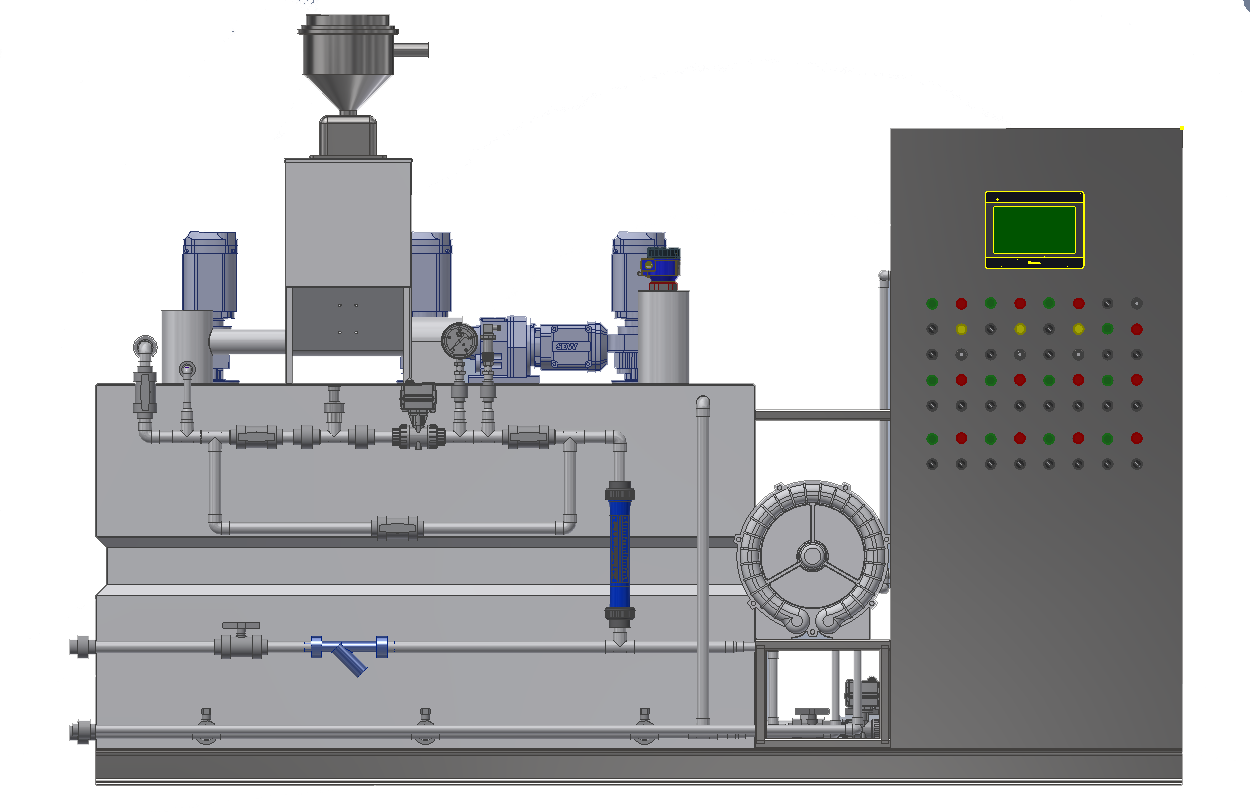
\includegraphics[height=10cm]{g9.PNG}};

                    %说明
                    \node at (-7,2) (2) [text_box] {进水流量探头};
                    \draw [arrow] (2) -- (-3.5,0);
                    \draw (-3.5,0) circle (0.5)[red];
                    \node at (0,3) (1) [text_box] {检修截止阀};
                    \draw [arrow] (1) -- (-1.2,-0.4);
                    \draw (-1.2,-0.4) circle (0.5)[red];
                    \node at (-8,-3) (3) [text_box] {检修旁通阀};
                    \draw [arrow] (3) -- (-2.7,-1.5);
                    \draw (-2.7,-1.5) circle (0.5)[red];
                    \node at (-8,1) (4) [text_box] {检修截止阀};
                    \draw [arrow] (4) -- (-4.5,-0.4);
                    \draw (-4.5,-0.4) circle (0.5)[red];
                    \node at (-6,3) (5) [text_box] {进水电动阀};
                    \draw [arrow] (5) -- (-2.5,0);
                    \draw (-2.5,0) circle (0.5)[red];
                    \node at (-1,4) (6) [text_box] {进水压力表及变送器};
                    \draw [arrow] (6) -- (-1.8,0.8);
                    \draw (-1.8,0.8) circle (0.5)[red];
                    \node at (3,5) (7) [text_box] {超声波液位计};
                    \draw [arrow] (7) -- (0.5,1.5);
                    \draw (0.5,1.5) circle (0.5)[red];
                    \node at (5,4) (8) [text_box] {超声波液位计安装座};
                    \draw [arrow] (8) -- (0.5,0.5);
                    \draw (0.5,0.5) circle (0.5)[red];

                    %辅助线
                    % \draw (-8,-5) [help lines] grid (8,5);
                    % \draw [red] (-8,0) -- (8,0);
                    % \draw [red] (0,-5) -- (0,5);
                \end{tikzpicture}
                \caption{主要传感器及电动阀位置}
            \end{figure}

            \par 检修进水流量探头、
            进水电动阀、
            进水压力表、
            进水压力变送器之前,
            应先关闭上下游检修截止阀,
            并打开检修旁通阀。
            \par 拆下
            超声波液位计安装座, 
            即可检修
            超声波液位计。

            \begin{figure}[h]
                \centering
                \begin{tikzpicture}
                    %图片
                    \node  at (0,0) {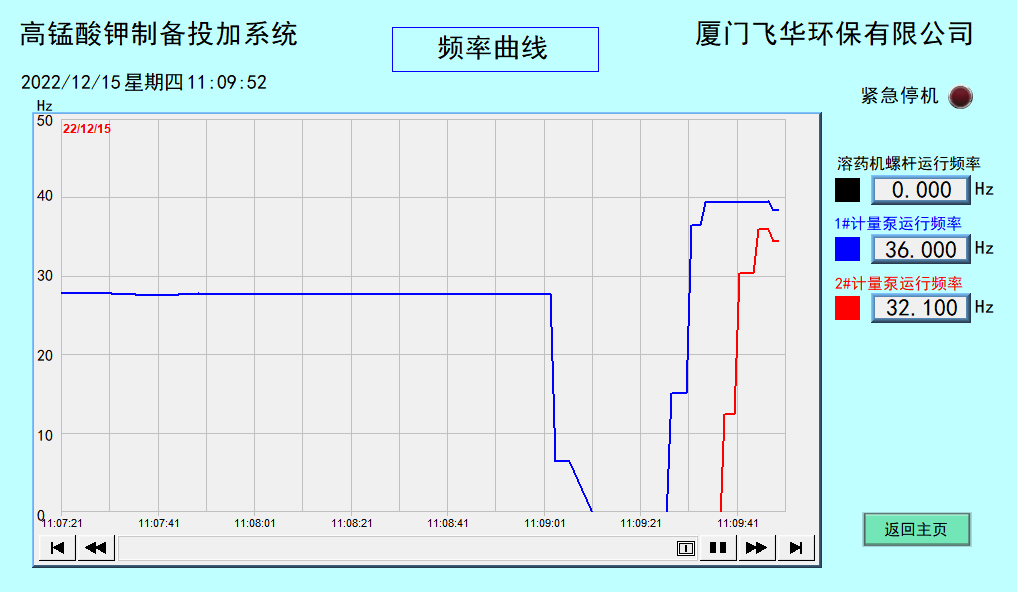
\includegraphics[height=5.5cm]{g10.PNG}};

                    %说明
                    \node at (-5,2) (2) [text_box] {料斗高料位探头};
                    \draw [arrow] (2) -- (0.5,2.2);
                    \draw (0.5,2.2) circle (0.5)[red];
                    \node at (-5,-1) (1) [text_box] {料斗低料位探头};
                    \draw [arrow] (1) -- (0.5,-0.2);
                    \draw (0.5,-0.2) circle (0.5)[red];

                    %辅助线
                    % \draw (-8,-2) [help lines] grid (8,2);
                    % \draw [red] (-8,0) -- (8,0);
                    % \draw [red] (0,-2) -- (0,2);
                \end{tikzpicture}
                \caption{料斗高低料位探头}\label{fig:g18}
            \end{figure}

            \par 料斗高低料位探头
            位置如上图\ref{fig:g18}所示。
            更换
            料斗高低料位探头
            之前,
            应先清理料斗内残留的高锰酸钾固体粉料。

            \newpage
        
        \subsubsection{搅拌机及螺旋进料器检修维护}
            检修维护搅拌机及螺旋进料器,
            特别是从装置上拆卸以及重新安装,
            有可能要打开制备系统的上盖,
            操作上较为复杂,
            建议联系加药系统经销商及售后服务人员处理。

            \begin{figure}[h]
                \centering
                \begin{tikzpicture}
                    %图片
                    \node  at (0,0) {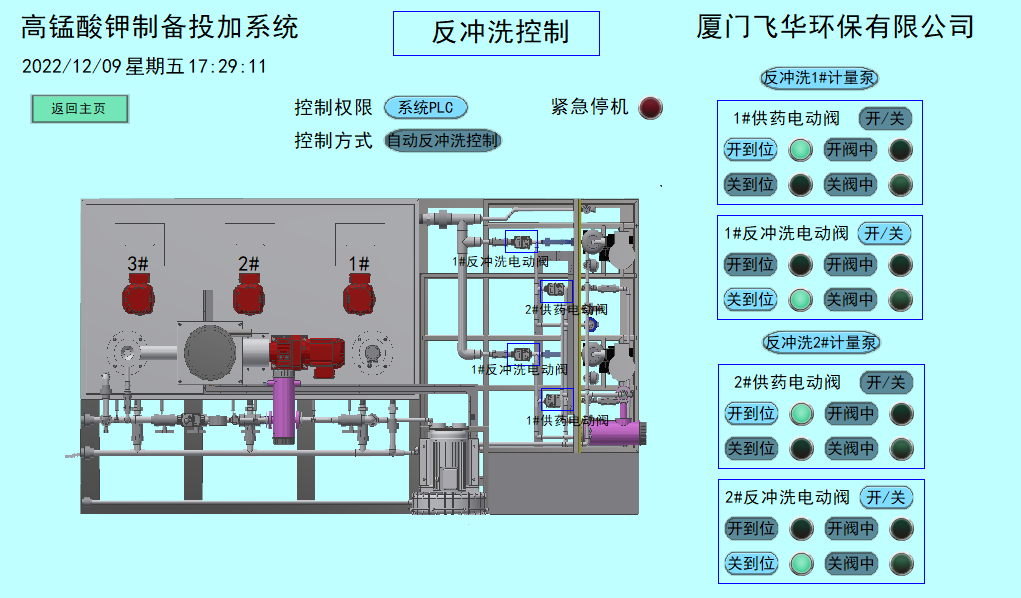
\includegraphics[height=10cm]{g3.PNG}};

                    %说明
                    \node at (4,-3) (2) [text_box] {排液阀};
                    \draw [arrow] (2) -- (1.2,-2);
                    \draw (1.2,-2) circle (0.5)[red];
                    \node at (3,-4) (1) [text_box] {排液阀};
                    \draw [arrow] (1) -- (-0.2,-2.8);
                    \draw (-0.2,-2.8) circle (0.5)[red];
                    \node at (2,-5) (3) [text_box] {排液阀};
                    \draw [arrow] (3) -- (-1.6,-3.5);
                    \draw (-1.6,-3.5) circle (0.5)[red];
                    \node at (-6,1) (4) [text_box] {连接活接};
                    \draw [arrow] (4) -- (-2.3,-0.8);
                    \draw (-2.3,-0.8) circle (0.5)[red];

                    %辅助线
                    % \draw (-8,-5) [help lines] grid (8,5);
                    % \draw [red] (-8,0) -- (8,0);
                    % \draw [red] (0,-5) -- (0,5);
                \end{tikzpicture}
                \caption{料斗高低料位探头}\label{fig:g19}
            \end{figure}

            \par 拆卸检修搅拌机及螺旋进料器之前,
            应先打开上图\ref{fig:g19}所示排液阀,
            排尽制备装置内液体,
            松开上图\ref{fig:g19}所示活接,
            才能打开制备系统上盖,
            检修或维护。

   \subsection{投加系统的检修维护}
        投加系统主要由
        计量泵、计量泵附件、流量探头、自动反冲洗系统组成。
        \par 上述设备均有2套各自独立,1用1备的系统,
        检修维护其中1套系统,
        不影响另外1套系统工作,
        满足高锰酸钾7*24小时投加的要求。
        \par 如果只是计量泵的阀球阀座之类卡了小型异物,
        可以只启动自动反冲洗系统,
        将小型异物冲走,
        不必拆卸维修。

        \subsubsection{关闭供药阀}
            检修前,
            应关闭检修工位的供药阀,
            防止储液槽内的高锰酸钾溶液,
            自流至检修工位范围内。
            \par 如果只是使用自动反冲洗系统,
            反冲洗管道,
            可跳过此步。

            \newpage
            
            \begin{figure}[h]
                \centering
                \begin{tikzpicture}
                    %图片
                    \node [rotate=-90] at (0,0) {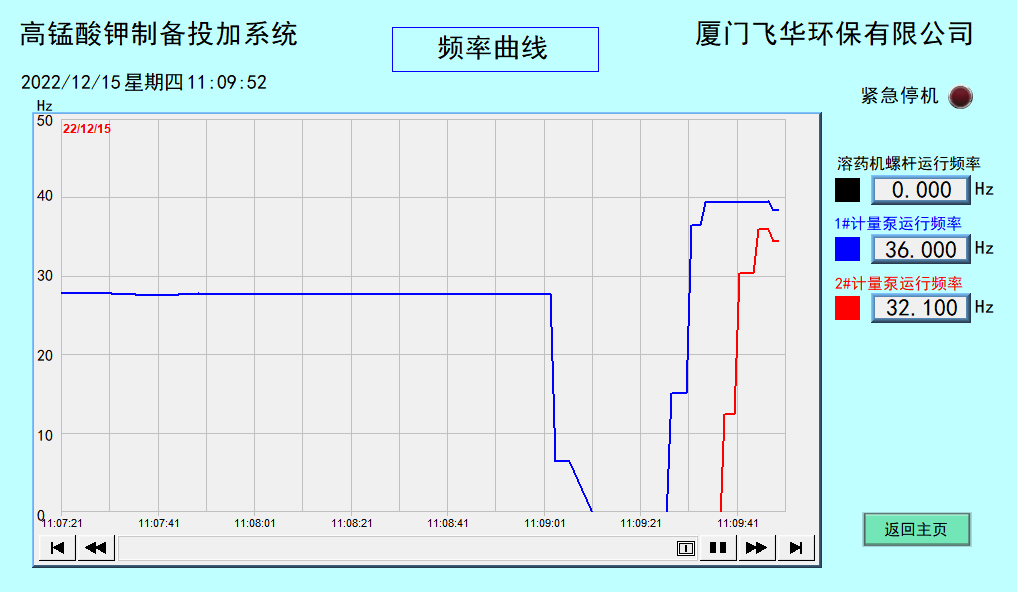
\includegraphics[height=9cm]{g10.PNG}};

                    %说明
                    \node at (-6,1) (1) [text_box] {供药阀};
                    \draw [arrow] (1) -- (-3.6,-0.8);
                    \draw (-3.6,-0.8) circle (0.5)[red];
                    \node at (-6,-4) (2) [text_box] {供药阀};
                    \draw [arrow] (2) -- (-2.5,-2.5);
                    \draw (-2.5,-2.5) circle (0.5)[red];

                    %辅助线
                    % \draw (-8,-5) [help lines] grid (8,5);
                    % \draw [red] (-8,0) -- (8,0);
                    % \draw [red] (0,-5) -- (0,5);
                \end{tikzpicture}
                \caption{供药阀位置}
            \end{figure}

        \subsubsection{反冲洗管道}
            投加系统配备自动反冲洗系统,
            进行检修维护之前,
            应启动自动反冲洗系统冲洗管道内化学品,
            再进行检修操作。
            \par  如果只是计量泵的阀球阀座之类卡了小型异物,
            可以只启动自动反冲洗系统,
            即可解决故障。
            \par 反冲洗过程完全自动,
            在人机界面上操作即可,
            操作过程如下图和图所示。

        \newpage

            \begin{figure}[h]
                \centering
                \begin{tikzpicture}
                    %图片
                    \node at (0,0) {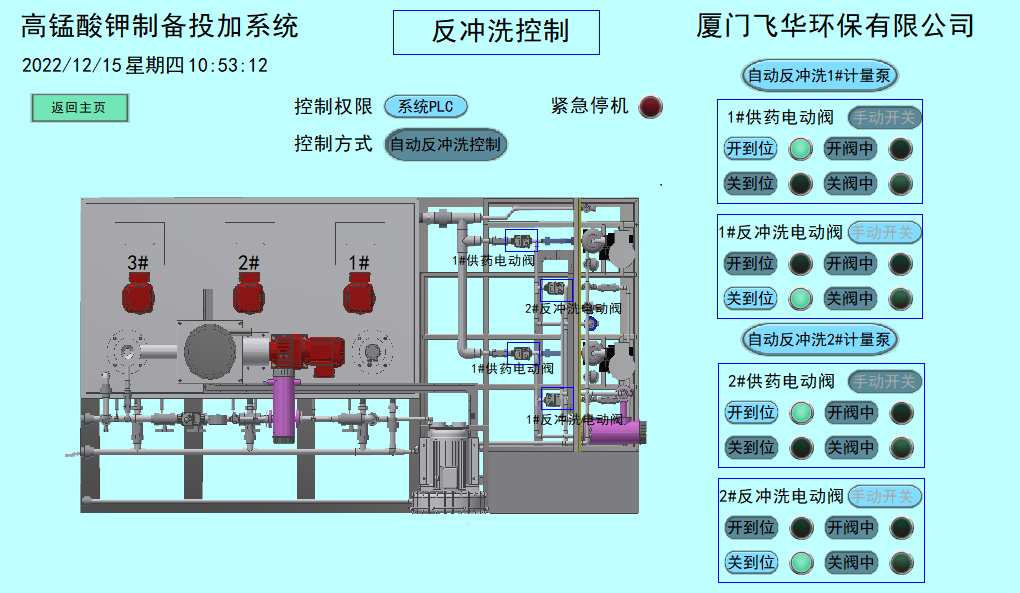
\includegraphics[height=8cm]{g6.PNG}};

                    %说明
                    \node at (-2,3) (1) [text_box, color=red] {自动反冲洗};
                    \draw (-3.5,2.1) rectangle +(1.5,0.6)[red];

                    %辅助线
                    % \draw (-8,-4) [help lines] grid (8,4);
                    % \draw [red] (-8,0) -- (8,0);
                    % \draw [red] (0,-4) -- (0,4);
                \end{tikzpicture}
                \caption{主控制界面}

                \vspace{6pt}

                \begin{tikzpicture}
                    %图片
                    \node at (0,0) {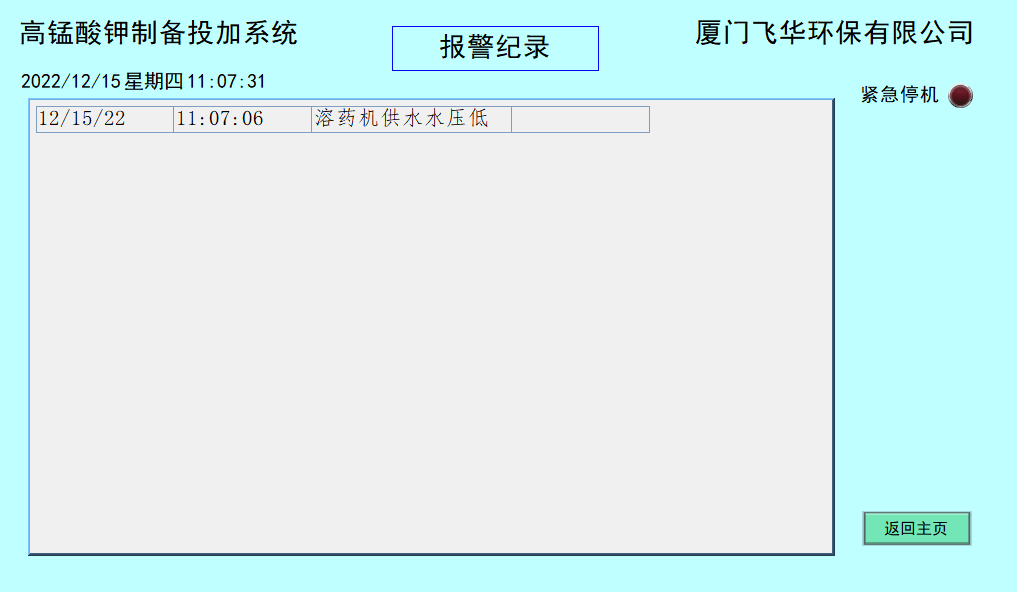
\includegraphics[height=8cm]{g8.PNG}};

                    %说明
                    \node at (6,3) (1) [text_box, color=red] {反冲1};
                    \node at (6,-0.6) (2) [text_box, color=red] {反冲2};
                    \draw (3.8,-0.9) rectangle +(1.8,0.5)[red];
                    \draw (3.8,2.6) rectangle +(1.8,0.5)[red];

                    %辅助线
                    % \draw (-8,-4) [help lines] grid (8,4);
                    % \draw [red] (-8,0) -- (8,0);
                    % \draw [red] (0,-4) -- (0,4);
                \end{tikzpicture}
                \caption{反冲洗控制按钮}
            \end{figure}

            \newpage

        \subsubsection{关闭相应工位的加药阀}
            检修前,
            应关闭检修工位的加药阀,
            防止下游管道内的化学品,
            回流至检修工位范围内。
            
            \begin{figure}[h]
                \centering
                \begin{tikzpicture}
                    %图片
                    \node [rotate=-90] at (0,0) {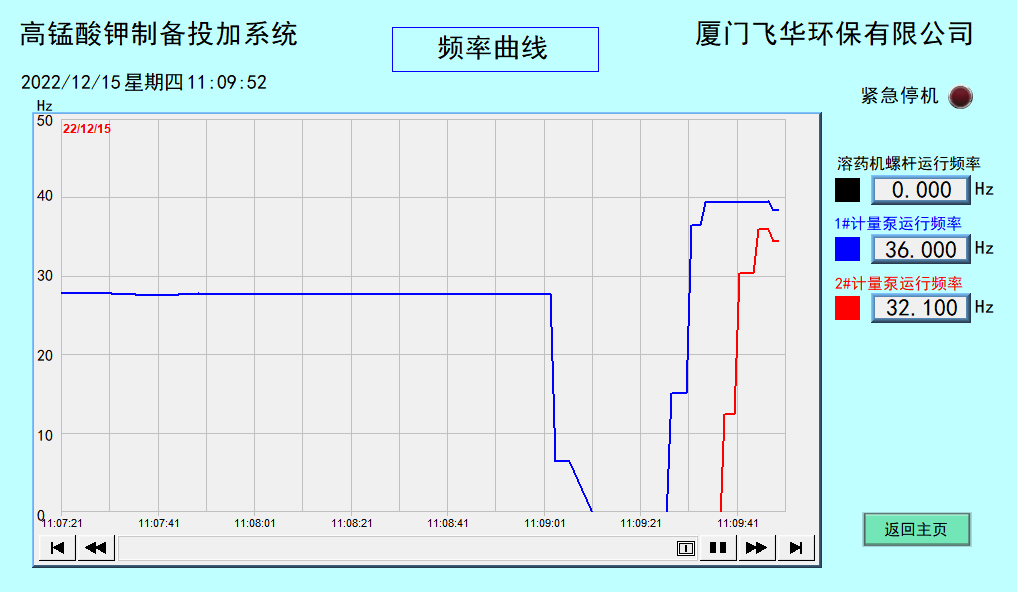
\includegraphics[height=9cm]{g10.PNG}};

                    %说明
                    \node at (-6,5) (1) [text_box] {加药阀};
                    \draw [arrow] (1) -- (-2,3.8);
                    \draw (-2,3.8) circle (0.5)[red];
                    \node at (6,5) (2) [text_box] {加药阀};
                    \draw [arrow] (2) -- (0.6,3.7);
                    \draw (0.6,3.7) circle (0.5)[red];
                    \node at (-6,-1) (3) [text_box] {排液阀};
                    \draw [arrow] (3) -- (-1.2,-0.2);
                    \draw (-1.2,-0.2) circle (0.5)[red];
                    \node at (6,-1) (4) [text_box] {排液阀};
                    \draw [arrow] (4) -- (1.2,-1.7);
                    \draw (1.2,-1.7) circle (0.5)[red];

                    %辅助线
                    % \draw (-8,-6) [help lines] grid (8,6);
                    % \draw [red] (-8,0) -- (8,0);
                    % \draw [red] (0,-6) -- (0,6);
                \end{tikzpicture}
                \caption{供药阀位置}\label{fig:g20}
            \end{figure}

        \subsubsection{打开相应工位的检修排液阀}
            \large{
                \textbf{
                    进行所有维护操作之前,
                    请先打开相应工位的检修排液阀,
                    释放系统内的压力!
                    否则,拆卸相关零部件时,
                    管道内的液体可能会喷射而出,
                    影响维修人员的安全!
                }
            }

            \par\normalsize{检修排液阀所在位置如上图\ref{fig:g20}所示。}

    \subsubsection{检修设备}
        待检修工位管道内残留化学品排净后,
        可对计量泵、阻尼器、隔膜压力表、背压阀、泄压阀、Y型过液器等设备或元件进行检修操作。
        \par 各设备或元件的检修方法,
        请参阅各设备或元件的使用说明,
        或咨询加药系统经销商或售后服务人员。

   \subsection{系统恢复运行}
        设备检修完成后,
        请关闭相应工位的检修排液阀,
        打开加药阀,
        打开供药阀,
        将投加系统的阀门都恢复至正常位置。
        \par 然后,
        请参阅第\ref{sec:sg1}章内容于第\pageref{sec:sg1}页,
        做好设备启动前准备,
        使系统处于待命状态,
        随时恢复正常运行。




\end{document}